% Präambel
\documentclass[%
fontsize=12pt,					% Schriftgröße
paper=a4,						% Papierformat
twoside=true, 					% einseitiges (false) oder zweiseitiges (true) Dokument
listof=totoc, 					% Tabellen- und Abbildungsverzeichnis ins Inhaltsverzeichnis
bibliography=totoc,				% Literaturverzeichnis ins Inhaltsverzeichnis aufnehmen
titlepage, 						% Titlepage-Umgebung statt \maketitle
headsepline, 					% horizontale Linie unter Kolumnentitel
%abstracton,					% Überschrift beim Abstract einschalten, Abstract muss dazu in {abstract}-Umgebung stehen
DIV=12,							% Satzspiegeleinstellung, 12 ist Standar bei KOMA
BCOR=6mm,						% Bindekorrektur, die den Seitenspiegel um 3mm nach rechts verschiebt,
cleardoublepage=empty,			% Stil einer leeren eingefügten Seite bei Kapitelwechsel
parskip,							% Absatzabstand bei Absatzwechsel einfügen
ngerman
]{scrbook}			
\usepackage[setspace=false]{scrhack}
\usepackage[utf8]{inputenc} 	% ermöglicht die direkte Eingabe von Umlauten
\usepackage[T1]{fontenc} 		% Ausgabe aller zeichen in einer T1-Codierung (wichtig für die Ausgabe von Umlauten!)
\usepackage{babel} 	% deutsche Trennungsregeln und Übersetzung der festcodierten Überschriften
\renewcaptionname{ngerman}{\contentsname}{Inhaltsverzeichnis}
\renewcaptionname{ngerman}{\bibname}{Literaturverzeichnis}
\setlength{\parindent}{0ex} 	% bei neuem Abschnitt nicht einrücken
%------
% Folgende Einstellungen entsprechen den Vorgaben der Leitlinien
\usepackage[onehalfspacing]{setspace}
% Ende Leitlinien
%------
%------
% Folgende Einstellungen sind bei größeren Arbeiten mit viel Text zu empfehlen.
% Hierbei oben DIV=16 einstellen und Zeile \usepackage[onehalfspacing]{setspace} auskommentieren.
%\linespread{1.2}\selectfont     % Zeilenabstand erhöhen - größere Werte als 1.2 nicht verwenden!!
% Ende Einstellung große Arbeiten mit viel Text.
%------

\newcommand{\lowrule}{%
	\leavevmode \kern.06em\vbox{\hrule width.5em}}

\usepackage{siunitx}			% Vereinfachte Eingabe von Einheiten in Formeln
\sisetup{
	number-unit-product = \;,
	inter-unit-product = \:,
	exponent-product = \cdot,
	output-decimal-marker = {,}
}

\usepackage{graphicx}  			% Einbinden von Grafiken erlauben
\usepackage[format=hang,		% Formatierungen von Unter- / Überschriften
font=normal,
labelfont=bf,
justification=RaggedRight,
singlelinecheck=true,
aboveskip=1mm
]{caption}

\usepackage[backend=biber, %% Hilfsprogramm "biber" beim Compilieren nutzen (statt "biblatex" oder "bibtex")
style=alphabetic, %% Zitierstil (siehe Dokumentation)
natbib=true, %% Bereitstellen von natbib-kompatiblen Zitierkommandos
hyperref=true, %% hyperref-Paket verwenden, um Links zu erstellen
]{biblatex}
\setcounter{biburllcpenalty}{7000}
\setcounter{biburlucpenalty}{8000}
\addbibresource{literature/literatur1.bib} %% Einbinden der bib-Datei. Endung .bib unbedingt ergänzen
\addbibresource{literature/literatur2.bib} %% Einbinden mehrerer bib-Dateien mit zusätzlichem \addbibresource - Befehl

\usepackage[normalem]{ulem}
\usepackage{csquotes}

% Folgende Zeilen sind auszukommentieren, falls runde Klammern und ein vgl. bei Zitaten erscheinen sollen.
%\makeatletter
%\renewcommand{\@cite}[2]{(vgl. {#1\if@tempswa , #2\fi})} 
%\renewcommand{\@biblabel}[1]{(#1)}
%\makeatother

\usepackage{pdfpages}

\usepackage{enumitem}			% Erlaubt Änderung der Nummerierung in der Umgebung enumerate

\usepackage{amsmath}			% Ergänzungen für Formeln
\usepackage{textcomp} 			% zum Einsatz von Eurozeichen u. a. Symbolen
\usepackage{eurosym}			% bessere Darstellung Euro-Symbol mit \euro

\usepackage[					% Einstellunge Paket hyperref
hyperfootnotes=false,			% im pfd-Output Fußnoten nicht verlinken
hidelinks						% Entfernen von farbigen Umrandungen der Links
]{hyperref}

\usepackage{makeidx}			% Paket zur Erstellung eines Index
\usepackage[toc]{glossaries}			% Paket zur Erstellung eines Glossars
\newglossaryentry{gls:glossar}
{
	name=Glossar,
	description={Als Glossar wird eine Liste von ausgewählten Begriffen bezeichnet, denen eine jeweilige Erläuterung zugeordnet ist. Ein Glossar wird, sofern gewünscht, im Anhang des Dokuments hinzugefügt.}
}
\usepackage[intoc]{nomencl} 			% zur Erstellung des Abkürzungsberzeichnisses

\usepackage[					% Einstellungen für Fußnoten
bottom,							% Ausrichtung unten
multiple,						% Trennung durch Seperator bei mehreren Fußnoten
hang,
marginal
]{footmisc}

\usepackage{calc}				% Paket zum Berechnen von Längen z.B. 0.8\linewidth

\usepackage{xcolor} 			% einfache Verwendung von Farben in nahezu allen Farbmodellen

\usepackage{listings}			% Darstellung von Quellcode mit den Umgebungen {lstlisting}, \lstinline und \lstinputlisting
\lstset{literate=				% Damit können Umlaute innerhalb Listings geschrieben werden
	{Ö}{{\"O}}1
	{Ä}{{\"A}}1
	{Ü}{{\"U}}1
	{ß}{{\ss}}1
	{ü}{{\"u}}1
	{ä}{{\"a}}1
	{ö}{{\"o}}1
}
\definecolor{mygreen}{rgb}{0,0.6,0}
\definecolor{mygray}{rgb}{0.5,0.5,0.5}
\definecolor{mymauve}{rgb}{0.58,0,0.82}
\lstset{ %
	backgroundcolor=\color{white},   % choose the background color; you must add \usepackage{color} or \usepackage{xcolor}; should come as last argument
	basicstyle=\footnotesize,        % the size of the fonts that are used for the code
	breakatwhitespace=false,         % sets if automatic breaks should only happen at whitespace
	breaklines=true,                 % sets automatic line breaking
	captionpos=t,                    % sets the caption-position to (b) bottom or (t) top
	commentstyle=\color{mygreen},    % comment style
	deletekeywords={...},            % if you want to delete keywords from the given language
	escapeinside={\%*}{*)},          % if you want to add LaTeX within your code
	escapeinside={(*@}{@*)},
	extendedchars=true,              % lets you use non-ASCII characters; for 8-bits encodings only, does not work with UTF-8
	frame=none,	                   	% "single" adds a frame around the code; "none"
	keepspaces=true,                 % keeps spaces in text, useful for keeping indentation of code (possibly needs columns=flexible)
	keywordstyle=\color{blue},       % keyword style
	language=[LaTeX]TeX,             % the language of the code
	morekeywords={*,nomenclature},   % if you want to add more keywords to the set
	numbers=left,                    % where to put the line-numbers; possible values are (none, left, right)
	numbersep=5pt,                   % how far the line-numbers are from the code
	numberstyle=\tiny\color{mygray}, % the style that is used for the line-numbers
	rulecolor=\color{black},         % if not set, the frame-color may be changed on line-breaks within not-black text (e.g. comments (green here))
	showspaces=false,                % show spaces everywhere adding particular underscores; it overrides 'showstringspaces'
	showstringspaces=false,          % underline spaces within strings only
	showtabs=false,                  % show tabs within strings adding particular underscores
	stepnumber=1,                    % the step between two line-numbers. If it's 1, each line will be numbered
	stringstyle=\color{mymauve},     % string literal style
	tabsize=2,	                   % sets default tabsize to 2 spaces
	title=\lstname                   % show the filename of files included with \lstinputlisting; also try caption instead of title
}

% -----------------------------------------------------------------------------------------------------------------
% Zum Aktualisieren des Abkürzungsverzeichnisses (Nomenklatur) bitte auf der Kommandozeile folgenden Befehl aufrufen :
% makeindex <Dateiname>.nlo -s nomencl.ist -o <Dateiname>.nls
% Oder besser: Kann in TexStudio unter Tools-Benutzer als Shortlink angelegt werden
% Konfiguration unter: Optionen-Erzeugen-Benutzerbefehle: makeindex -s nomencl.ist -t %.nlg -o %.nls %.nlo
% -----------------------------------------------------------------------------------------------------------------

% Hier die persönlichen Daten eingeben:

\newcommand{\titel}{Titel der Projekt- / Studien- / Haus- oder Bachelorarbeit}
\newcommand{\untertitel}{ggf. Untertitel mit ergänzenden Hinweisen}
\newcommand{\arbeit}{Projektarbeit T3\lowrule 1000 / Projektarbeit T3\lowrule 2000 / Studienarbeit T3\lowrule 3100 / Hausarbeit T3\lowrule 3000 / Studienarbeit T3\lowrule 3200 / Bachelorarbeit T3\lowrule 3300}
\newcommand{\studiengang}{Elektrotechnik}
\newcommand{\studienrichtung}{Fahrzeugelektronik}
\newcommand{\studienschwerpunkt}{}
\newcommand{\autor}{Autorin / Autor}
\newcommand{\bearbeitungszeitraum}{01.01.2024 - 31.03.2024}
\newcommand{\matrikelnr}{123 456}
\newcommand{\kurs}{TFE23-2}
\newcommand{\firma}{Name des Dualen Partners (entfällt ggf. bei Studienarbeit)}
\newcommand{\abgabe}{\today}
\newcommand{\betreuerfirma}{Betreuerin / Betreuer der Arbeit}
\newcommand{\gutachterdhbw}{Gutachterin / Gutachter der DHBW (nur bei Bachelorarbeit)}

\newcommand{\jahr}{2019}			% für Angabe im Copyright-Vermerk der Titelseite

% Folgende Zeilen definieren Abkürzungen, um Befehle schneller eingeben zu können
\newcommand{\ua}{\mbox{u.\,a.\ }}
\newcommand{\zB}{\mbox{z.\,B.\ }}
\newcommand{\bs}{$\backslash$}
\newcommand*\diff{\mathop{}\!\mathrm{d}}	% Differentialzeichen
\newcommand*\Diff[1]{\mathop{}\!\mathrm{d^#1}} % Differentialzeichen höherer Ableitung
\newcommand*\jj{\mathop{}\!\mathrm{j}}	% Komplexe Zahl j

% Folgende Zeilen weden benötigt, um Tikz und PGF-Plot-Grafiken einzubinden
\usepackage{pgfplots}
\usepackage{pgfplotstable}
\pgfplotsset{compat=newest,width=0.6\linewidth}
\usepgfplotslibrary{smithchart}
\usepackage{tikz}						% Tikz sollte nach Listings Pakete geladen werden.
\usetikzlibrary{arrows}

\hyphenation{Schrift-ar-ten}

\BeforeClosingMainAux{% siehe KOMA-Script-Anleitung
\addcontentsline{toc}{chapter}{\indexname}\stepcounter{page}
}

\makeindex						% Indexverzeichnis erstellen
\makenomenclature				% Abkürzungsverzeichnis erstellen
\makeglossaries

% -------------------------------------------------------------------------------------------
%                     Beginn des Dokumenteninhalts
% -------------------------------------------------------------------------------------------
\begin{document}
\let\texteuro\euro						% Eingabe \texteuro, € oder \euro erzeugt gleiches Ergebnis
\setcounter{secnumdepth}{3}				% Nummerierungstiefe fürs Inhaltsverzeichnis
\setcounter{tocdepth}{3}
\sffamily								% für die Titelei serifenlose Schrift verwenden

% ------------------------------ Titelei -----------------------------------------------------

\thispagestyle{plain}
\hypersetup{pageanchor=false}
\begin{titlepage}
\enlargethispage{4.0cm}
\sffamily 								% Serifenlose Grundschrift für die Titelseite einstellen

\parbox{0.5\linewidth}{
\begin{flushleft}
% Hier ggf. ein Logo der Firma
\end{flushleft}
}
\parbox{0.5\linewidth}{
\begin{flushright}
	
\includegraphics[width=0.4\linewidth]{images/DHBW_d_R_FN_46mm_4c}\\[5ex]
\end{flushright}
}
				

\begin{center}

{\fontsize{20.74pt}{24pt}\selectfont
\textbf{\titel}\\[1.5ex]}
{\fontsize{14pt}{17pt}\selectfont
\textbf{\untertitel}\\[5ex]}
{\fontsize{17pt}{20pt}\selectfont
\textbf{\arbeit}\\[2ex]}
{\fontsize{14pt}{17pt}\selectfont
Studiengang \studiengang\\[2ex]}
{\fontsize{12pt}{14pt}\selectfont
Studienrichtung \studienrichtung\\[1ex]
Duale Hochschule Baden-Württemberg Ravensburg, Campus Friedrichshafen\\[5ex]
von\\[1ex]
\autor\\[15ex]}


\end{center}

\begin{flushleft}
{\fontsize{12pt}{14pt}\selectfont
\begin{tabular}{ll}
Abgabedatum:					& \quad \abgabe \\
Bearbeitungszeitraum:		   	& \quad \bearbeitungszeitraum   \\ 
Matrikelnummer: 			& \quad \matrikelnr \\ 
Kurs: 							& \quad \kurs \\
%Dualer Partner:	 			& \quad \firma \\ % entfällt bei Studienarbeit
Betreuerin / Betreuer:  & \quad \betreuerfirma \\ % Betreuerin / Betreuer der Arbeit
%Gutachterin / Gutachter: & \quad \gutachterdhbw \\ [2ex] % Gutachterin / Gutachter der DHBW (nur bei der Bachelorarbeit erforderlich)
\end{tabular}
}
\end{flushleft}
%%%%% Nachfolgende Zeilen einkommentieren, wenn Copyrightvermerk gewünscht ist
%\begin{flushleft}
%{\fontsize{11pt}{13pt}\selectfont
%Copyrightvermerk:\\
%Dieses Werk einschließlich seiner Teile ist \textbf{urheberrechtlich geschützt}. Jede Verwertung außerhalb der engen Grenzen des Urheberrechtgesetzes ist ohne Zustimmung des Autors unzulässig und strafbar. Das gilt insbesondere für Vervielfältigungen, Übersetzungen, Mikroverfilmungen sowie die Einspeicherung und Verarbeitung in elektronischen Systemen.
%}
%\end{flushleft}
%\begin{flushright}
%{\fontsize{11pt}{13pt}\selectfont \copyright{} \jahr }
%\end{flushright}
\end{titlepage}

\ifthenelse{\boolean{@twoside}}{%
	\cleardoublepage
}{%
	\clearpage
}%

\hypersetup{pageanchor=true}
 				% erzeugt die Titelseite
\pagenumbering{roman}					% kleine, römische Seitenzahlen für Titelei
% Ggf. folgende Zeile auskommentieren, falls der Sperrvermerk gewünscht ist.
\chapter*{Sperrvermerk} %*-Variante sorgt dafür, das der Sperrvermerk nicht im Inhaltsverzeichnis auftaucht
gemäß Ziffer 1.1.14 der Anlage 1 zu §§ 3, 4 und 5  der Studien- und Prüfungsordnung für die Bachelorstudiengänge im Studienbereich Technik der Dualen Hochschule Baden-Württemberg vom 29.09.2017 in der Fassung vom 24.07.2023:

Der Inhalt dieser Arbeit darf weder als Ganzes noch in Auszügen Personen außerhalb des Prüfungsprozesses und des Evaluationsverfahrens zugänglich gemacht werden, sofern keine anders lautende Genehmigung vom Dualen Partner vorliegt.

Friedrichshafen, den \today \\[4ex]

\rule[-0.2cm]{10cm}{0.5pt} \\

\textsc{\autor} \\[10ex]

\chapter*{Erklärung} %*-Variante sorgt dafür, dass die Erklärung nicht im Inhaltsverzeichnis auftaucht

gemäß Ziffer 1.1.14 der Anlage 1 zu §§ 3, 4 und 5  der Studien- und Prüfungsordnung für die Bachelorstudiengänge im Studienbereich Technik der Dualen Hochschule Baden-Württemberg vom 29.09.2017 in der Fassung vom 24.07.2023.

Ich versichere hiermit, dass ich meine \arbeit\ mit dem Thema:

\begin{quote}
	\textit{\titel} % -\textit{ \untertitel }
\end{quote}

selbstständig verfasst und keine anderen als die angegebenen Quellen und Hilfsmittel benutzt habe. Ich versichere zudem, dass die eingereichte elektronische Fassung mit der gedruckten Fassung übereinstimmt.\\[6ex]

Musterstadt, den \today \\[1ex]

\rule[-0.2cm]{5cm}{0.5pt} \\

\autor \\[10ex]

\rmfamily

\thispagestyle{empty}

 				% Einbinden der eidestattlichen Erklärung
\chapter*{Kurzfassung} %*-Variante sorgt dafür, das Abstract nicht im Inhaltsverzeichnis auftaucht

%*******************************************************************************************************************
Aufgrund des Fachkräftemangels, auch im Bereich Logistik, wird es immer wichtiger, möglich viele Arbeitsschritte zu automatisieren.
In dieser Hausarbeit wird einer fiktiven Optimierung eines Hochregallagers nachgegangen. 
Momentan befindet sich das Hochregal in einem kompletten manuellen Betrieb. Die Ware muss von einem Mitarbeiter händisch einsortiert werden. Dieser pflegt auch die Daten ins System ein und bestellt bei Bedarf die Ware nach.
All diese Arbeitsschritte sind zeitintensiv und anfällig für Fehler.
%-----------------------------------Problemstellung---------------------------------------------------------------
Ziel ist es, durch eine Automatisierung soll das Hochregallager effizienter werden. Die Automatisierung soll zu einer höheren Produktivität führen, indem die Bearbeitungszeit verringert und die Fehler minimiert werden. Dafür soll das Hochregalsystem in der Lage sein, die Waren eigenständig ein- und auslagern zu können. 
Bei einem niedrigen Lagerbestand soll über das ERP-System neue Ware nachbestellt werden. Hierfür ist es notwendig, dass das Hochregallager den Lagerbestand in Echtzeit überwacht. Um diese Anforderung umzusetzen, ist es wichtig, dass alle Produkte zuverlässig erkannt werden. Die Erkennung erfolgt über die RFID-Technologie, welche eine hohe Digitalisierung des Lagers voraussetzt, um die Informationen kontinuierlich aktualisieren zu können.
%-----------------------------------Zielsetzung---------------------------------------------------------------------
%% Der Absatz gefällt mir noch nicht 
Ziel dieser Hausarbeit ist es, ein umfassendes Grobkonzept zu entwickeln. Dieses Konzept soll dabei helfen, die Idee eines automatisierten Hochregallagers klar und anschaulich der Geschäftsleitung zu präsentieren. 
Das Aufzeigen der Vorteile soll die Manager von einer Umstellung auf eine Automation überzeugen und die Bereitstellung eines Budgets sichern.



\chapter*{Abstract} %*-Variante sorgt dafür, das Abstract nicht im Inhaltsverzeichnis auftaucht

English translation of the \glqq Kurzfassung\grqq.

\clearpage   			% Einbinden des Abstracts

\tableofcontents						% Erzeugen des Inhalsverzeichnisses

\clearpage

% --------------------------------------------------------------------------------------------
%                    Inhalt der Bachelorarbeit
%---------------------------------------------------------------------------------------------
\pagenumbering{arabic}					% arabische Seitenzahlen für den Hauptteil

\rmfamily

\chapter{Einleitung}

%*******************************************************************************************************************
Aufgrund des Fachkräftemangels, auch im Bereich Logistik, wird es immer wichtiger, möglich viele Arbeitsschritte zu automatisieren.
In dieser Hausarbeit wird einer fiktiven Optimierung eines Hochregallagers nachgegangen. 
Momentan befindet sich das Hochregal in einem kompletten manuellen Betrieb. Die Ware muss von einem Mitarbeiter händisch einsortiert werden. Dieser pflegt auch die Daten ins System ein und bestellt bei Bedarf die Ware nach.
All diese Arbeitsschritte sind zeitintensiv und anfällig für Fehler.

%-----------------------------------Problemstellung---------------------------------------------------------------
Ziel ist es, durch eine Automatisierung soll das Hochregallager effizienter werden. Die Automatisierung soll zu einer höheren Produktivität führen, indem die Bearbeitungszeit verringert und die Fehler minimiert werden. Dafür soll das Hochregalsystem in der Lage sein, die Waren eigenständig ein- und auslagern zu können. 
Bei einem niedrigen Lagerbestand soll über das ERP-System neue Ware nachbestellt werden. Hierfür ist es notwendig, dass das Hochregallager den Lagerbestand in Echtzeit überwacht. Um diese Anforderung umzusetzen, ist es wichtig, dass alle Produkte zuverlässig erkannt werden. Die Erkennung erfolgt über die RFID-Technologie, welche eine hohe Digitalisierung des Lagers voraussetzt, um die Informationen kontinuierlich aktualisieren zu können.

%-----------------------------------Zielsetzung---------------------------------------------------------------------
														%% Der Absatz gefällt mir noch nicht 
Ziel dieser Hausarbeit ist es, ein umfassendes Grobkonzept zu entwickeln. Dieses Konzept soll dabei helfen, die Idee eines automatisierten Hochregallagers klar und anschaulich der Geschäftsleitung zu präsentieren. 
Das Aufzeigen der Vorteile soll die Manager von einer Umstellung auf eine Automation überzeugen und die Bereitstellung eines Budgets sichern.

%-----------------------------------Gliederung---------------------------------------------------------------------
In dieser Hausarbeit wird auf folgende fünf Themen eingegangen:
\begin{enumerate}
	\item \textbf{Benefits: }Hier wird auf die Vorteile, welche durch eine Automatiesierung des Lagers entstehen, eingegangen
	\item \textbf{Vorgehensweise:}
	\item \textbf{Risiken:} Im Kapitel über Risiken werden die technologischen, wirtschaftlichen und Sicherheitsaspekte eingehend analysiert und reflektiert.
	\item \textbf{Kosten:}
	\item \textbf{Innovationsgrad:}
\end{enumerate}
\chapter{Grundlagen}
\label{cha:Grundlagen}

Zielgerichtete theoretische Grundlagen, sowohl fachliche, wie auch methodische.

Zu den Grundlagen gehören z.~B. auch Details zur Problemstellung, der Stand der Technik und weitere Grundlagen, welche zur Konzeptausarbeitung, Umsetzung und Verifikation erforderlich sind.

Grundlagen haben immer einen Bezug zu den nachfolgenden Kapiteln. Diesen Bezug sollte man gelegentlich explizit herstellen, damit bereits in diesem Kapitel klar ist, wo und für was die Grundlagen gebraucht und angewandt werden.
\chapter{Vorgehen}
\label{cha:vorgehen}

Je nach Art der Arbeit kann diese Kapitelüberschrift auch \glqq Konzeptentwurf\grqq~lauten.

Beschreibung der Ausgangssituation und des Themenumfelds. Ggf. wird darauf eingegangen, welche Randbedingungen und Einflüsse zu beachten sind.

Anforderungsanalyse und Anforderungsdefinition, nach Möglichkeit strukturiert, um zu einem späteren Zeitpunkt die Anforderungen nachvollziehbar verifizieren zu können.

Herleitung einer Lösung (einer Methodik, eines experimentellen Aufbaus oder von unterschiedlichen Konzepten), Lösungsbewertung und bewusste Wahl des gewählten Vorgehens. An dieser Stelle ist auch auf die Zuverlässigkeit einer Methodik oder auf die Genauigkeit von Untersuchungen einzugehen. Die Überlegungen sollen dazu helfen, mit der angestrebten Lösung die gestellten Anforderungen zu erfüllen, um schließlich die Ziele der Arbeit erreichen zu können.

Bei einer Gegenüberstellung von verschiedenen Lösungsansätzen kann z.~B. eine Nutzwertanalyse helfen. Dabei sind nicht nur z.~B. die Funktion, Leistungsfähigkeit, Umsetzbarkeit und Nutzbarkeit, sondern auch z.~B. wirtschaftliche Aspekte, wie Stück-, Entwicklungskosten oder Ressourcenverbrauch zu berücksichtigen. Sehr bedeutend sind auch Aspekte der Nachhaltigkeit unter Betrachtung des gesamten Lebenszyklus einer erarbeiteten Lösung.

Sowohl bei der Anforderungsdefinition, als auch bei der Lösungsfindung gibt es eine große Anzahl an verschiedenen Methoden. Eine kleine Auswahl ist in der folgenden Aufzählung zu finden.

\begin{itemize}
\item Anforderungsdefinition mithilfe des Requirements Engineering  \autocite{Pohl.2021}
\item Systems Engineering Ansatz \autocite{Schluter.2023}
\item Agile Entwicklungsmethodiken \autocite{Cohn.2010, Martin.2020, Wirdemann.2022}
\item Klassische Bewertungsverfahren \autocite{Breiing.1997, Zangemeister.2014}
\end{itemize}

Ziel dieses Kapitels ist, dass auf Basis von umfassend und genau formulierten Anforderungen (ggf. auch Nicht-Zielen) eine Lösungsvielfalt erarbeitet wird, welche anschließend strukturiert bewertet wird, um eine fundierte Begründung für die angestrebte Art der Umsetzung herzuleiten.
\chapter{Umsetzung und Ergebnisse}
\label{cha:umsetzung}

Je nach Art der Arbeit kann diese Kapitelüberschrift auch \glqq Ergebnisse\grqq~lauten, z.~B. bei rein messtechnischen Aufgaben.

Beschreibung der Umsetzung des zuvor gewählten Vorgehens (theoretische Untersuchung, Erhebungen, Durchführung von Experimenten, Prototypenaufbau, Implementierung eines Prozesses, etc.).

Verifikation anhand der zuvor erarbeiteten Anforderungen und Validierung in Bezug auf das zuvor gestellte Ziel. Diskussion der Ergebnisse. Spätestens hier auch auf die Zuverlässigkeit der gewonnenen Erkenntnisse eingehen (z.~B. anhand der Genauigkeit von Messergebnissen).
\chapter{Zusammenfassung}

Die Kombination aus WMS, ERP und den automatisierten Regalbediengeräten schafft ein vollständig integriertes, „smartes“ Lager. Alle Prozesse laufen digital gesteuert ab, was nicht nur die Geschwindigkeit und Präzision der Lagerprozesse erhöht, sondern auch die Datentransparenz und Steuerbarkeit im gesamten Unternehmen verbessert.
Die Automatisierung des Hochregallagers bietet eine erhebliche Chance, die Effizienz zu steigern und die Betriebskosten nachhaltig zu senken. Der derzeitige manuelle Prozess mit Gabelstaplern und händischer Dateneingabe verursacht hohe Personalkosten und Fehlerkosten. Durch die Implementierung eines automatisierten Systems, das Regalbediengeräte, Förderbänder und ein Lagerverwaltungssystem umfasst, werden diese ineffizienten Prozesse deutlich reduziert.

Die jährlichen Einsparungen von etwa 380.000 € durch geringeren Personalaufwand und reduzierte Fehler- und Betriebskosten ermöglichen es, die Investitionskosten von 2.025.000 € in weniger als 5,5 Jahren zu amortisieren. Nach dieser Amortisationszeit wird das Unternehmen langfristig von den Einsparungen profitieren. Darüber hinaus erhöht die Automatisierung nicht nur die Effizienz, sondern auch die Sicherheit, da der Einsatz von Gabelstaplern und damit das Unfallrisiko minimiert wird.

Die Investition in die Automatisierung ist daher eine wirtschaftlich vorteilhafte Entscheidung, die sowohl die Wettbewerbsfähigkeit steigert als auch zu einer erheblichen Kostenersparnis führt.

% ---- Literaturverzeichnis ----------
\interlinepenalty 10000					% Verhindert einen Umbruch mitten in Literatureinträgen
\printbibliography						% Erstellen des Literaturverzeichnisses
\interlinepenalty 0
\clearpage

% -----Ausgabe aller Verzeichnisse ---
\setlength{\parskip}{0.5\baselineskip}

% Alle Abkürzungen, die in der Arbeit verwendet werden. Die Alphabetische Sortierung übernimmt Latex. Nachfolgend sind Beispiele genannt, welche nach Bedarf angepasst, gelöscht oder ergänzt werden können.
% Die Angaben in der eckigen Klammer werden zur Sortierung der Einträge verwendet. Vor allem bei Formelzeichen hat man sonst das Problem, dass diese möglicherweise nicht wie gewünscht sortiert werden.

% Bei den unten stehenden Formelzeichen ist erläutert, wie explizite Sortierschlüssel über den Inhalt der eckigen Klammer angegeben werden.

% Zum Aktualisieren des Abkürzungsverzeichnisses (Nomenklatur) bitte auf der Kommandozeile folgenden Befehl aufrufen :
% makeindex <Dateiname>.nlo -s nomencl.ist -o <Dateiname>.nls
% Oder besser: Kann in TexStudio unter Tools-Benutzer als Shortlink angelegt werden
% Konfiguration unter: Optionen-Erzeugen-Benutzerbefehle: makeindex -s nomencl.ist -t %.nlg -o %.nls %.nlo

% Allgemeine Abkürzungen %%%%%%%%%%%%%%%%%%%%%%%%%%%%
%\nomenclature[Abb]{Abb.}{Abbildung}
%\nomenclature[bzw]{bzw.}{beziehungsweise}
%\nomenclature[DHBW]{DHBW}{Duale Hochschule Baden-Württemberg}
%\nomenclature[ebd]{ebd.}{ebenda}
%\nomenclaturev[etal]{et al.}{at alii}
\nomenclature[etc]{etc.}{et cetera}
%\nomenclature[evtl]{evtl.}{eventuell}
\nomenclature[f]{f.}{folgende Seite}
\nomenclature[ff]{ff.}{fortfolgende Seiten}
%\nomenclature[ggf]{ggf.}{gegebenenfalls}
%\nomenclature[Hrsg]{Hrsg.}{Herausgeber}
%\nomenclature[Tab]{Tab.}{Tabelle}
%\nomenclature[ua]{u. a.}{unter anderem}
%\nomenclature[usw]{usw.}{und so weiter}
\nomenclature[vgl]{vgl.}{vergleiche}
\nomenclature[zB]{z. B.}{zum Beispiel}
%\nomenclaturev[zT]{z. T.}{zum Teil}

% Dateiendungen %%%%%%%%%%%%%%%%%%%%%%%%%%%%%%%%%%%%
\nomenclature[EMF]{EMF}{Enhanced Metafile}
\nomenclature[JPG]{JPG}{Joint Photographic Experts Group}
\nomenclature[KI]{KI}{Künstliche Intelligenz}
\nomenclature[PDF]{PDF}{Portable Document Format}
\nomenclature[PNG]{PNG}{Portable Network Graphics}
%\nomenclature[]{XML}{Extensible Markup Language}

% Abkürzungen von Fachbegriffen %%%%%%%%%%%%%%%%%%%%
\nomenclature[ABS]{ABS}{Antiblockiersystem}
\nomenclature[ESC]{ESC}{Electronic Stability Control, Fahrdynamikregelung}

% Formelzeichen %%%%%%%%%%%%%%%%%%%%%%%%%%%%%%%%%%%%
\nomenclature[a]{$a$}{Beschleunigung}
\nomenclature[F]{$F$}{Kraft}
\nomenclature[m]{$m$}{Masse}
\nomenclature[P]{$P$}{Leistung}
\nomenclature[U]{$U$}{Spannung}
\nomenclature[R]{$R$}{Widerstand}


				% Datei mit allgemeinen Abkürzungen laden
\renewcommand{\nomname}{Verzeichnis verwendeter Formelzeichen und Abkürzungen}
%\addcontentsline{toc}{chapter}{\nomname}
\setlength{\nomlabelwidth}{.20\hsize}
\renewcommand{\nomlabel}[1]{#1 \dotfill}
\setlength{\nomitemsep}{-\parsep}
\printnomenclature						% Erzeugen des Abkürzungsverzeichnises, siehe auch Inhalt der Datei pages/abkuerzungen.tex
\clearpage

\listoffigures 							% Erzeugen des Abbildungsverzeichnisses 
\clearpage

\listoftables 							% Erzeugen des Tabellenverzeichnisses
\clearpage

% -----Anhang ------------------------

\appendix
%\pagenumbering{Roman}					% große, römische Seitenzahlen für Anhang, falls gewünscht
\addchap{A Nutzung von Künstliche Intelligenz basierten Werkzeugen}
\setcounter{chapter}{1}

Im Rahmen dieser Arbeit wurden Künstliche Intelligenz (KI)\index{Künstliche Intelligenz} basierte Werkzeuge benutzt. Tabelle~\ref{tab:anhang_uebersicht_KI_werkzeuge} gibt eine Übersicht über die verwendeten Werkzeuge und den jeweiligen Einsatzzweck.

\begin{table}[hbt]	
	\centering
	\renewcommand{\arraystretch}{1.5}	% Skaliert die Zeilenhöhe der Tabelle
	\captionabove[Liste der verwendeten Künstliche Intelligenz basierten Werkzeuge]{Liste der verwendeten KI basierten Werkzeuge}
	\label{tab:anhang_uebersicht_KI_werkzeuge}
	\begin{tabular}{>{\raggedright\arraybackslash}p{0.3\linewidth} >{\raggedright\arraybackslash}p{0.65\linewidth}}
		\textbf{Werkzeug} & \textbf{Beschreibung der Nutzung}\\
		\hline 
		\hline
		ChatGPT & 	\vspace{-\topsep}
					\begin{itemize}[noitemsep,topsep=0pt,partopsep=0pt,parsep=0pt] 
						\item Grundlagenrecherche zu bekannten Prinzipien optischer Sensorik zur Abstandsmessung (siehe Abschnitt \ldots)
						\item Suche nach Herstellern von Lidar-Sensoren (siehe Abschnitt \ldots)
						\item \ldots
				   	\end{itemize} \\
		ChatPDF &	\vspace{-\topsep}
					\begin{itemize}[noitemsep,topsep=0pt,partopsep=0pt,parsep=0pt] 
					\item Recherche und Zusammenfassung von wissenschaftlichen Studien im Themenfeld \ldots
					\item \ldots
					\end{itemize} \\ 
		DeepL	&	\vspace{-\topsep}
					\begin{itemize}[noitemsep,topsep=0pt,partopsep=0pt,parsep=0pt] 
					\item Übersetzung des Papers von $[\ldots]$
					\end{itemize} \\ 
		Tabnine AI coding assistant &	\vspace{-\topsep}
							\begin{itemize}[noitemsep,topsep=0pt,partopsep=0pt,parsep=0pt] 
							\item Aktiviertes Plugin in MS Visual Studio zum Programmieren des \ldots
							\item \ldots
							\end{itemize} \\ 
		\ldots	&	\vspace{-\topsep}
					\begin{itemize}[noitemsep,topsep=0pt,partopsep=0pt,parsep=0pt] 
					\item \ldots
					\end{itemize} \\ 
		\hline 
	\end{tabular} 
\end{table}

\addchap{B Ergänzungen}
\setcounter{chapter}{2}

\section{Details zu bestimmten theoretischen Grundlagen}

\section{Weitere Details, welche im Hauptteil den Lesefluss behindern}

\addchap{C Details zu Laboraufbauten und Messergebnissen}
\setcounter{chapter}{3}
\setcounter{section}{0}
\setcounter{table}{0}
\setcounter{figure}{0}

\section{Versuchsanordnung}

\section{Liste der verwendeten Messgeräte}

\section{Übersicht der Messergebnisse}

\section{Schaltplan und Bild der Prototypenplatine}

\addchap{D Zusatzinformationen zu verwendeter Software}
\setcounter{chapter}{4}
\setcounter{section}{0}
\setcounter{table}{0}
\setcounter{figure}{0}

\section{Struktogramm des Programmentwurfs}

\section{Wichtige Teile des Quellcodes}

\addchap{E Datenblätter}
\setcounter{chapter}{5}
\setcounter{section}{0}
\setcounter{table}{0}
\setcounter{figure}{0}

%\section{Einbinden von PDF-Seiten aus anderen Dokumenten}

Auf den folgenden Seiten wird eine Möglichkeit gezeigt, wie aus einem anderen PDF-Dokument komplette Seiten übernommen werden können, z.~B. zum Einbindungen von Datenblättern. Der Nachteil dieser Methode besteht darin, dass sämtliche Formateinstellungen (Kopfzeilen, Seitenzahlen, Ränder, etc.) auf diesen Seiten nicht angezeigt werden. Die Methode wird deshalb eher selten gewählt. Immerhin sorgt das Package \textit{\glqq pdfpages\grqq}~für eine korrekte Seitenzahleinstellung auf den im Anschluss folgenden \glqq nativen\grqq~\LaTeX-Seiten.

Eine bessere Alternative ist, einzelne Seiten mit \textit{\glqq$\backslash$includegraphics\grqq}~einzubinden.


\includepdf[pages={2-4}]{docs/EingebundenesPDF.pdf}

\clearpage

\clearpage

\addchap{F Tips und Beispiele zu \LaTeX-Befehlen}
\setcounter{chapter}{6}
\setcounter{section}{0}
\setcounter{table}{0}
\setcounter{figure}{0}

Dieses Kapitel können Sie einfach löschen, indem Sie in der Präambel am Anfang der Zeile \glqq \textbackslash\textit{include\{chapter/anhang\lowrule vorlagen\}}\grqq~das Symbol \% zum Auskommentieren einfügen.

\section{Wichtige \LaTeX -Befehle}

\begin{tabbing}
\hspace*{0cm} \= \hspace{0.42\linewidth} \= \+\kill
\textbackslash \textit{label}\{\}	\> Definition eines Labels, auf welches referenziert \\ 
	\> werden kann, z.~B.: \textbackslash \textit{label}\{fig:MyImage\}\\ 
\textbackslash \textit{ref}\{\}	\> Setzen einer Referenz zu einem Label\\
\> z.~B.: \ldots siehe Tabelle\~{}\textbackslash \textit{ref}\{tab:messdaten\}.\\ 
\textbackslash \textit{pageref}\{\}	\> Gibt die Seitenzahl zu einer Referenz zurück\\

	\textbackslash \textit{autocite}\{\}	\> Literaturreferenz einfügen\\
	\textbackslash \textit{autocite}[7]\{\}	\> Literaturreferenz einfügen, hier mit zus. Referenz\\
	\> auf Seite 7\\
\textbackslash \textit{autocites}\{Abc15, Def16\}	\> Mehrere Literaturreferenzen, hier Abc15 und \\
\> Def16, einfügen\\
\textbackslash \textit{footnote}\{\}	\> Fußnote einfügen\\ 
\~{}	\> Einfügen eines geschützten Leerzeichens\\ 
\textdollar \textit{Formel} \textdollar	\> Eingabe einer Formel im Text\\
\textdollar\textit{l}=\textbackslash \textit{SI}\{10\}\{\textbackslash \textit{meter}\}\textdollar	\> Korrekte Ausgabe Maßzahl und Einheit in\\
\> Formeln, hier $l=\SI{10}{\meter}$\\
\textbackslash \textit{index}\{Kraft\} \> Aufnahme des Begriffs \glqq Kraft\grqq~in das Sachwort- \index{Kraft} \\
\> verzeichnis\\
\textbackslash \textit{index}\{Induktion!Vollständige\} \> Aufnahme des Begriffs \glqq Vollständige\grqq~in das Sach-\\
\> wortverzeichnis unter \glqq Induktion\grqq. \index{Induktion!Vollständige} \\
\textbackslash \textit{nomenclature}[etc]\{etc.\}\{et cetera\}	\> Aufnahme der Abkürzung \glqq etc.\grqq~für \glqq et cetera\grqq~in \\
\> das Abkürzungsverzeichnis. Die Angabe [etc] dient\\
\>als Sortierschlüssel\\
\textbackslash \textit{clearpage}	\> Ausgabe aller Gleitobjekte und Umbruch auf eine\\
\> neue Seite\\ 
\end{tabbing}

\clearpage

\section{Vorlagen für \LaTeX Umgebungen}

\subsection{Listen und Aufzählungen}

Es gibt folgende Listentypen. Die wichtigsten:

\begin{itemize}
	\item Einfache Liste mit \textit{itemize}-Umgebung
	\item ...
\end{itemize}

\begin{enumerate}
	\item Nummerierte Liste mit \textit{enumerate}-Umgebung
	\item ...
\end{enumerate}

\begin{enumerate}[label=\alph*.]
	\item wobei man bei der \textit{enumerate}-Umgebung leicht die Art der Nummerierung ändern kann,
	\item ...
\end{enumerate}

und durch verschachtelte Umgebungen verschiedene Aufzählungsebenen darstellen kann:

\begin{enumerate}[label=\alph*)]
	\item Erster Aufzählungspunkt der ersten Ebene
	\item ...
	\begin{itemize}
		\item Erster Punkt der zweiten Ebene
		\item Zweiter Punkt der zweiten Ebene
	\end{itemize}
	\item Das sollte an Beispielen zunächst einmal genügen.
\end{enumerate}

\clearpage

\subsection{Bilder und Grafiken}

Bilder können als PDF-, JPG-, und PNG-Bilder in \LaTeX eingebunden werden. Damit eine Grafik in hoher Qualität dargestellt wird, sollte das Dateiformat der Grafik vektorbasiert sein, d.h. als PDF-Datei vorliegen. Viele Zeichenprogramme unterstützen einen PDF-Export (z.~B. GIMP, Adobe Illustrator, etc.). Für Grafiken aus PowerPoint sei folgende Vorgehensweise beim Export empfohlen:

\begin{enumerate}
	\item Die gewünschte Grafik in PowerPoint zeichnen.
	\item Gewünschten Bildbereich markieren, rechte Maustaste klicken und \glqq Als Grafik speichern ...\grqq~wählen.
	\item Grafik im Format EMF abspeichern. Das EMF-Format ist vektorbasiert.\footnote{Mit dem Mac kann in PowerPoint die Grafik direkt im PDF-Format exportiert werden. Die weiteren Schritte entfallen daher.}
	\item Mit dem Programm XnView die Grafik im EMF-Format in PDF wandeln und abspeichern.
	\item Die so erzeugte PDF-Datei enthält eine vektorbasierte Grafik und kann in \LaTeX~ eingebunden werden.
\end{enumerate}

Abbildung~\ref{fig:MyImage} zeigt ein Beispielbild einer Grafik, welche aus PowerPoint exportiert wurde.

\begin{figure}[hbt]
	\centering
	
\includegraphics[width=0.3\linewidth]{images/MyImage}
	\caption[Beispiel für die Einbindung eines Bildes.]{Beispiel für die Einbindung eines Bildes (PDF-, JPG-, und PNG-Bilder können eingebunden werden).}
	\label{fig:MyImage}
\end{figure}

Der Quellcode des Beispielbildes aus Abbildung~\ref{fig:MyImage} ist in Listing~\ref{lst:fig} zu sehen.

\clearpage

\begin{lstlisting}[caption=Quellcode der Abbildung~\ref{fig:MyImage}.,label=lst:fig]
\begin{figure}[hbt]				% here, bottom, top
\centering						% Zentrierung

\includegraphics[width=0.6\linewidth]{images/MyImage}		
\caption[Beispiel für die Einbindung eines Bildes.]{Beispiel für die Einbindung eines Bildes (PDF-, JPG-, und PNG-Bilder können eingebunden werden).}
\label{fig:MyImage}
\end{figure}
\end{lstlisting}

Jedes Bild aus fremder Quelle ist mit einem Zitat in der Abbildungsunterschrift zu kennzeichnen. Nur eigene Bilder benötigen keine entsprechende Kennzeichnung. Bilder aus fremder Quelle mit eigenen Ergänzungen oder Änderungen sind mit Zitat und einer entsprechenden Bemerkung (z. B. \glqq auf Basis [Quelle] mit eigenen Ergänzungen\grqq~oder \glqq eigene Darstellung auf Basis [Quelle]\grqq) zu versehen. Der besseren Lesbarkeit halber sind im Abbildungsverzeichnis keine Zitate anzugeben. Hierfür kann im Befehl \textbackslash \textit{caption[]\{\}} innerhalb der eckigen Klammer eine modifizierte Abbildungsunterschrift eingegeben werden, welche in das Abbildungsverzeichnis übernommen wird. Der Text innerhalb der geschweiften Klammer wird direkt unter die Abbildung gedruckt und kann dagegen ausführlich mit Angabe eines Zitats sein. Sollte die Arbeit veröffentlicht werden, ist unbedingt darauf zu achten, dass nur dann Bilder von fremder Quelle übernommen werden dürfen, wenn hierfür das explizite Einverständnis des Urhebers vorliegt. Dieses Einverständnis ist persönlich einzuholen und separat zu dokumentieren.

Grafiken können auch mithilfe des Packages Tikz gezeichnet, bzw. programmiert werden. Grafiken mit Tikz werden mit dem \textit{input}-Befehl in die \textit{figure}-Umgebung geladen, wie nachfolgendes Beispiel in Abbildung~\ref{fig:tikz_house} zeigt:

\begin{figure}[hbt]
	\centering
	 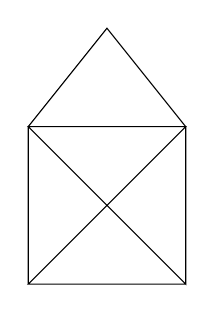
\begin{tikzpicture}
\draw (0,0) -- (0,2) -- (1,3.25) -- (2,2) -- (2,0) -- (0,2) -- (2,2) -- (0,0) -- (2,0);
\end{tikzpicture}
    
	\caption[Mit Tikz programmierte Grafik.]{Mit Tikz programmierte Grafik.}
	\label{fig:tikz_house}
\end{figure}

Ein etwas umfangreicheres Beispiel zur Digitaltechnik ist in Abbildung~\ref{fig:tikz_digital} dargestellt:

\begin{figure}[hbt]
	\centering
	\usetikzlibrary{circuits.logic.US,circuits.logic.IEC}
      \begin{tikzpicture}[circuit logic US]
      \matrix[column sep=7mm]
      {
      \node (i0) {0}; & & \\
      & \node [and gate] (a1) {}; & \\
      \node (i1) {0}; & & \node [or gate] (o) {};\\
      & \node [nand gate] (a2) {}; & \\
      \node (i2) {1}; & & \\
      };
      \draw (i0.east) -- ++(right:3mm) |- (a1.input 1);
      \draw (i1.east) -- ++(right:3mm) |- (a1.input 2);
      \draw (i1.east) -- ++(right:3mm) |- (a2.input 1);
      \draw (i2.east) -- ++(right:3mm) |- (a2.input 2);
      \draw (a1.output) -- ++(right:3mm) |- (o.input 1);
      \draw (a2.output) -- ++(right:3mm) |- (o.input 2);
      \draw (o.output) -- ++(right:3mm) node [right] {$y$ \quad Hier könnte Ihre Formel $y=(0 \land 0) \lor \overline{( 0 \land 1)}$ stehen};
 \end{tikzpicture}

	\caption[Mit Tikz programmierte Grafik, welche bereits vorgefertigte Bibliotheken für Symbole aus der Digitaltechnik nutzt.]{Mit Tikz programmierte Grafik, welche bereits vorgefertigte Bibliotheken für Symbole aus der Digitaltechnik nutzt.}
	\label{fig:tikz_digital}
\end{figure}

%\clearpage

In der Tikz-Umgebung können auch Diagramme mit dem \textit{pgfplot}-Befehlssatz erzeugt werden. In Abbildung \ref{fig:pgfplot} sehen Sie ein Beispiel.

\begin{figure}[hbt]
	\centering
	\begin{tikzpicture}
		\begin{axis}[scale=1.3,legend entries={Messwerte mit Fehlerbalken,
			$\pgfmathprintnumber{\pgfplotstableregressiona} \cdot x  
			\pgfmathprintnumber[print sign]{\pgfplotstableregressionb}$}, legend style={draw=none},legend style={at={(0.01,0.98)},anchor=north west},xlabel=Stromstärke $I \; \mathrm{ \lbrack mA \rbrack}$,ylabel=Spannung $U \; \mathrm{ \lbrack V \rbrack}$]
		\addlegendimage{mark=*,blue}
		\addlegendimage{no markers,red}
\addplot+[error bars/.cd, y dir=both,y explicit]
table[x=x,y=y,y error=errory] 
{pgfplot/messdaten_mitfehler.dat};
\addplot table[mark=none,y={create col/linear regression={y=y}}]
{pgfplot/messdaten_mitfehler.dat};
	\end{axis}
\end{tikzpicture}
	\caption[Diagramm, erstellt mit dem \textit{pgfplot}-Befehlssatz.]{Ein Diagramm, erstellt in der \textit{tikzpicture}-Umgebung mit dem \textit{pgfplot}-Befehlssatz. Das Diagramm stellt Messdaten, deren Fehlerbalken und eine Regressionskurve dar. Die Messdaten werden von einer separaten Datei eingelesen und die Regressionskurve wurde mit \textit{pgfplot} berechnet und erstellt.}
	\label{fig:pgfplot}
\end{figure}

\clearpage

Auch hierzu der Quellcode in Listing~\ref{lst:pgfplot}.

\begin{lstlisting}[caption=Quellcode der Abbildung~\ref{fig:pgfplot}.,label=lst:pgfplot]
\begin{figure}[hbt]
\centering
\begin{tikzpicture}
		\begin{axis}[scale=1.3,legend entries={Messwerte mit Fehlerbalken,
			$\pgfmathprintnumber{\pgfplotstableregressiona} \cdot x  
			\pgfmathprintnumber[print sign]{\pgfplotstableregressionb}$}, legend style={draw=none},legend style={at={(0.01,0.98)},anchor=north west},xlabel=Stromstärke $I \; \mathrm{ \lbrack mA \rbrack}$,ylabel=Spannung $U \; \mathrm{ \lbrack V \rbrack}$]
		\addlegendimage{mark=*,blue}
		\addlegendimage{no markers,red}
\addplot+[error bars/.cd, y dir=both,y explicit]
table[x=x,y=y,y error=errory] 
{pgfplot/messdaten_mitfehler.dat};
\addplot table[mark=none,y={create col/linear regression={y=y}}]
{pgfplot/messdaten_mitfehler.dat};
	\end{axis}
\end{tikzpicture}
\caption[Diagramm, erstellt mit dem \textit{pgfplot}-Befehlssatz.]{Ein Diagramm, erstellt in der \textit{tikzpicture}-Umgebung mit dem \textit{pgfplot}-Befehlssatz. Das Diagramm stellt Messdaten, deren Fehlerbalken und eine Regressionskurve dar. Die Messdaten werden von einer separaten Datei eingelesen und die Regressionskurve wurde mit \textit{pgfplot} berechnet und erstellt.}
\label{fig:pgfplot}
\end{figure}
\end{lstlisting}

In Listing~\ref{lst:tikz} ist der Quellcode der Datei \textit{mess\_fehlerbalken.tex} dargestellt.

\begin{lstlisting}[caption=Quellcode der Datei \textit{mess\_fehlerbalken.tex}.,label=lst:tikz]
\begin{tikzpicture}
\begin{axis}[scale=1.3,legend entries={Messwerte mit Fehlerbalken,
$\pgfmathprintnumber{\pgfplotstableregressiona} \cdot x  
\pgfmathprintnumber[print sign]{\pgfplotstableregressionb}$}, legend style={draw=none},legend style={at={(0.01,0.98)},anchor=north west},xlabel=Stromstärke $I \; \mathrm{ \lbrack mA \rbrack}$,ylabel=Spannung $U \; \mathrm{ \lbrack V \rbrack}$]
\addlegendimage{mark=*,blue}
\addlegendimage{no markers,red}
\addplot+[error bars/.cd, y dir=both,y explicit]
table[x=x,y=y,y error=errory] 
{pgfplot/messdaten_mitfehler.dat};
\addplot table[mark=none,y={create col/linear regression={y=y}}]
{pgfplot/messdaten_mitfehler.dat};
\end{axis}
\end{tikzpicture}
\end{lstlisting}

\clearpage

In Abbildung~\ref{fig:pgfplot2y} wird ein weiters Beispiel für ein Diagramm gezeigt. Oftmals wird eine zweite y-Achse verwendet, um verschiedene Skalen darstellen zu können.

\begin{figure}[hbt]
	\centering
	\begin{tikzpicture}
%
\begin{axis}[
scale=1.3,
ytick pos=left,
xlabel=Zeit $t \; \mathrm{ \lbrack ns \rbrack}$,
ylabel=Spannung $U \; \mathrm{ \lbrack V \rbrack}$
]
\addplot[mark=*,only marks] table[x=x,y=y1] {pgfplot/messdaten_zweiyachsen.dat};
\end{axis}
%
\begin{axis}[
scale = 1.3,
legend style={draw=none},
legend style={at={(0.75,0.6)},
anchor=north west},
axis y line*=right,
axis x line=none,
%ymin=0,
%ymax=100,
ylabel=Strom $I \; \mathrm{ \lbrack mA \rbrack}$
]
\addlegendimage{mark=*,only marks}
\addlegendentry{Spannung}
\addplot[mark=x,only marks,blue] table[x=x,y=y2] {pgfplot/messdaten_zweiyachsen.dat};
\addlegendentry{Strom}
\end{axis}
\end{tikzpicture}
	\caption[Diagramm mit zwei unterschiedlichen y-Achsen.]{Diagramm mit zwei unterschiedlichen y-Achsen.}
	\label{fig:pgfplot2y}
\end{figure}

\clearpage

\subsection{Tabellen}

\begin{table}[hbt]	
	\centering
	\renewcommand{\arraystretch}{1.5}	% Skaliert die Zeilenhöhe der Tabelle
	\captionabove[Liste der verwendeten Messgeräte]{Liste der verwendeten Messgeräte. Die Genauigkeitsangaben beziehen sich auf die Standardabweichung $1\cdot \sigma$.}
	\label{tab:bsp}
	\begin{tabular}{ccccc}
		\textbf{Messgerät} & \textbf{Hersteller} & \textbf{Typ} & \textbf{Verwendung} & \textbf{Genauigkeit}\\ 
		\hline 
		\hline 
		\parbox[t]{0.2\linewidth}{\centering Spannungs-\\versorgung} & Voltmaker & HV2000 & \parbox[t]{0.2\linewidth}{\centering Spannungs-\\versorgung der\\Platine} & $\Delta U = \pm 5 $~mV \\ % Der parbox-Befehl ist erforderlich, damit ein Zeilenumbruch erzeugt werden kann. c-Spalten (zentriert) erlauben nicht automatisch einen Zeilenumpruch. Linksbündig gesetzte p-Spalten erlauben automatisch den Zeilenumbruch.
		Strommessgerät & Currentcount & Hotamp 16 & \parbox[t]{0.2\linewidth}{ \centering Strommessung\\am Versorgungspin\\des µC} & $\Delta I = \pm 0.1$~A \\ 
		\hline 
	\end{tabular} 
\end{table}

Der Quellcode der Beispieltabelle~\ref{tab:bsp} ist in Listing~\ref{lst:tab} zu sehen.

\begin{lstlisting}[caption=Quellcode der Tabelle~\ref{tab:bsp}.,label=lst:tab]
\begin{table}[hbt]	
\centering
\renewcommand{\arraystretch}{1.5}	% Skaliert die Zeilenhöhe der Tabelle
\captionabove[Liste der verwendeten Messgeräte]{Liste der verwendeten Messgeräte. Die Genauigkeitsangaben beziehen sich auf die Standardabweichung $1\cdot \sigma$.}
\label{tab:bsp}
\begin{tabular}{ccccc}
\textbf{Messgerät} & \textbf{Hersteller} & \textbf{Typ} & \textbf{Verwendung} & \textbf{Genauigkeit}\\ 
\hline 
\hline 
\parbox[t]{0.2\linewidth}{\centering Spannungs-\\versorgung} & Voltmaker & HV2000 & \parbox[t]{0.2\linewidth}{\centering Spannungs-\\versorgung der\\Platine} & $\Delta U = \pm 5 $~mV \\ % Der parbox-Befehl ist erforderlich, damit ein Zeilenumbruch erzeugt werden kann. c-Spalten (zentriert) erlauben nicht automatisch einen Zeilenumpruch. Linksbündig gesetzte p-Spalten erlauben automatisch den Zeilenumbruch.
Strommessgerät & Currentcount & Hotamp 16 & \parbox[t]{0.2\linewidth}{ \centering Strommessung\\ am Versorgungspin\\ des \textmu C} & $\Delta I = \pm 0.1$~A \\ 
\hline 
\end{tabular} 
\end{table}
\end{lstlisting}

\clearpage

\subsection{Formeln}

Formeln lassen sich in \LaTeX~ganz einfach schreiben. Es gibt unterschiedliche Umgebungen zum Schreiben von Formeln. Z.~B. direkt im Text $v=s/t$ oder abgesetzt

\[F=m \cdot a\]

oder auch, wie in wissenschaftlichen Dokumenten üblich, nummeriert

\begin{equation}
P=\frac{U^2}{R} \quad .
\label{eqn:leistung}
\end{equation}

Mit einem Label in Formel~\ref{eqn:leistung} lassen sich natürlich auch Formeln im Text referenzieren. \LaTeX~verwendet im Formelmodus einen eigenen Schriftsatz, welcher entsprechend der gängigen Konventionen kursive Zeichen verwendet. Sollen im Formelmodus Einheiten in normaler Schriftart eingefügt werden, dann kann dies über den Befehl \textbackslash \textit{mathrm}\{\} erwirkt werden, wie im Quellcode von Formel~\ref{eqn:leistungMitEinh} zu sehen ist.

\begin{equation}
P=\frac{U^2}{R} = \frac{\left( 100~\mathrm{V}\right)^2}{100~\Omega} = 100~\mathrm{W}\quad .
\label{eqn:leistungMitEinh}
\end{equation}

Zum direkten Vergleich sind die Einheiten in Formel~\ref{eqn:leistungMitEinhfalsch} falsch dargestellt:

\begin{equation}
P=\frac{U^2}{R} = \frac{\left( 100~V\right)^2}{100\,\varOmega} = 100\,W
\label{eqn:leistungMitEinhfalsch}
\end{equation}

Zur einfachen Eingabe von Einheiten kann auch das Package \textbackslash \textit{siunitx} verwendet werden:

\begin{equation}
	P=\SI{100}{\watt}=\SI{100}{\joule\per\second}
\end{equation}

Das sind nur ein paar wenige Beispiele und es gibt sehr viele Packages, um Besonderheiten in Formeln realisieren zu können, z.~B. mehrzeilige Formeln mit vertikaler Ausrichtung. Nennen Sie Formeln nur, wenn diese zum besseren Verständnis auch wirklich nützlich sind.

Folgende Befehle sind innerhalb von Formel-Umgebungen nützlich:
\begin{tabbing}
	\hspace*{0cm} \= \hspace{0.28\linewidth} \= \+\kill
	\textbackslash \textit{text}\{\} oder \textbackslash \textit{mathrm}\{\}	\> Damit kann in Formel-Umgebung Text geschrieben werden.\\ 
	\textbackslash, \textbackslash: \textbackslash; \textbackslash quad \textbackslash qquad \> Zusätzlichen Abstand zwischen Symbolen einfügen.\\
	\textbackslash \textit{notag} \> Nummerierung einer bestimmten Formel ausschalten.
\end{tabbing}

Hier noch ein kleines Beispiel aus der Mathematik:

\begin{equation}
\sum\limits_{n=1}^\infty f\left(x_n\right)\cdot \Delta x=  \lim\limits_{\Delta x \rightarrow 0} \frac{f\left(x_0+\Delta x\right)-f\left(x_0\right)}{\Delta x} = \frac{\diff f}{\diff x} = \dot{f}(x)
\end{equation}

Und abschließend ein Beispiel aus der Physik zum Induktionsgesetz\index{Induktion!Elektromagnetische}:

\begin{equation}
\oint \limits _{\partial {\mathcal {\mathcal {A}}}(t)}{{\vec {E}}\cdot {\text{d}}{\vec {s}}}=-\int \limits _{{\mathcal {A}}(t)}{{\frac {\partial {\vec {B}}}{\partial t}}\cdot {\text{d}}{\vec {A}}}
\end{equation}

		% Zeile auskommentieren bei finalem Dokument!


\renewcommand{\glossaryname}{Glossar}
\printglossaries
%\addcontentsline{toc}{chapter}{\glossaryname}

\renewcommand{\indexname}{Sachwortverzeichnis}
\printindex								% Erzeugen des Sachwortverzeichnisses

\end{document}